\documentclass[a4paper]{article}
\usepackage[utf8]{inputenc} % para poder usar tildes en archivos UTF-8
\usepackage[spanish]{babel} % para que comandos como \today den el resultado en castellano
\usepackage{a4wide} % márgenes un poco más anchos que lo usual
\usepackage[showRevisiones]{caratula}
\usepackage{xcolor}
\usepackage{listings}
\lstset{basicstyle=\ttfamily,
  showstringspaces=false,
  commentstyle=\color{red},
  keywordstyle=\color{blue}
}

\begin{document}

\materia{Organización de Computadoras 66.20}
\tipoapunte{Trabajo Práctico #1}

\fecha{\today}

\autor{Quino López, Julián}{94224}{julian.quino2@gmail.com}
\autor{Del Carril, Manuel}{100772}{manueldelcarril@gmail.com}
\autor{Bobadilla Catalan, German}{90123}{bobadillagerman@gmail.com}

\revision{07/05/2019}{-}{Entrega del TP}

\maketitle

\renewcommand{\abstractname}{Resumen} 
\begin{abstract}
El siguiente trabajo práctico tiene como objetivo familiarizarse con el conjunto de instrucciones MIPS y el concepto de ABI. Para lograr tal propósito se escribe en lenguaje assembly MIPS dos programas que permitan convertir archivos de texto desde Windows hacia UNIX, y viceversa.
\end{abstract}


\section{Introducción}
Los archivos de texto requieren de un carácter especial (o secuencia de caracteres) para indicar el fin de una línea. La codificación de este varía según el sistema operativo, lo que lleva a la incorrecta visualización de un archivo en un sistema operativo que fue creado en otro. Linux utiliza el salto de línea \verb|(\n)| mientras que Windows utiliza el retorno del carro seguido del salto de línea \verb|(\r\n)|.

\section{Desarrollo}

El algoritmo propuesto por el grupo consiste en recorrer caracter por caracter hasta encontrar un \verb|\r|, si el programa usado es dos2unix y el siguiente caracter es un \verb|\n| se eliminará el \verb|\r| , si en cambio se usa el programa unix2dos se agregara \verb|\r| antes de un \verb|\n|, esto se realiza ya sea desde el archivo o utilizando el stream leído por entrada standard.

\subsection{Implementación}

En ambos programas la implementación es similar, simplemente difieren en los caracteres que detectan y los que reemplazan. Por ende, la siguiente descripción servirá para ambos casos. Tenemos cuatro funcioes globales: myRead, myWrite, processInput y main, cada cual con tareas específicas.


myRead se encarga de leer los caracteres del documento y los devuelve, verificando previamente de que no haya errores. Por otro lado, myWrite funciona como myRead, solo que como su nombre lo indica, escribe un caracter en el documento.

processInput utiliza estas dos funciones para procesar el archivo caracter a caracter y escribir el resultado.

main es como su nombre indica, la función que inicia el programa y se encarga de recibir los comandos pasados por stdin y actuar en consecuencia, donde en caso de ser necesario llamará a processInput.


\subsection{Comandos para compilar y ejecutar el programa}

Se puede compilar los programas con los siguientes comandos:

\begin{lstlisting}[language=bash]
  $ gcc unix2dos.c -o unix2dos
  $ gcc dos2unix.c -o dos2unix
\end{lstlisting}


Y luego ejecutarlos con los comandos:

\begin{lstlisting}[language=bash]
  $ ./unix2dos -i input.txt -o output.txt
  $ ./dos2unix -i input.txt -o output.txt
\end{lstlisting}

En caso de sólo querer especificar el archivo de entrada, debe ejecutarse, por ejemplo, de la siguiente manera:

\begin{lstlisting}[language=bash]
  $ ./unix2dos -i input.txt -o -
  $ ./dos2unix -i input.txt -o -
\end{lstlisting}

Análogamente si se quiere ingresar un archivo de salida:

\begin{lstlisting}[language=bash]
  $ ./unix2dos -i - -o output.txt
  $ ./dos2unix -i - -o output.txt
\end{lstlisting}

Es decir que con un guión medio indicamos que no se proporcionará un archivo para entrada/salida, acorde a lo que indica el enunciado.

\subsection{Otros comandos}

Pueden utilizarse comandos tales como help y version, de la siguiente forma:

\begin{lstlisting}[language=bash]
  $ ./unix2dos -h
  $ ./dos2unix -h
\end{lstlisting}

\begin{lstlisting}[language=bash]
  $ ./unix2dos -V
  $ ./dos2unix -V
\end{lstlisting}

\subsection{Código fuente de unix2dos.S}
\lstset{breaklines=true}
\begin{lstlisting}[language=Assembler]
#include <mips/regdef.h>
#include <sys/syscall.h>

#define SALIDA_EXITOSA 0
#define ERROR -1
#define ARCHIVO_NULO -1
#define ENTRADA_ESTANDAR 0
#define SALIDA_ESTANDAR 1
	#int myRead(char *buffer,int cantidad,file)
	.text
	.align	2
	.globl	myRead
	.ent	myRead
myRead:
	.frame	$fp,32,ra
	.set	noreorder
	.cpload	t9
	.set	reorder

	subu	sp,sp,32
	.cprestore  16
	sw		$fp,20(sp)
	move	$fp,sp
	sw		ra,12($fp)

	move	t0,a1
	move	a1,a0
	move	a0,a2
	move	a2,t0
	li		v0,SYS_read
	syscall
	#vemos si hay errores primero
	bne		a3, zero, ErrorEnRead
	bgt		zero,v0, ErrorEnRead
	b		salidaDeMyRead
ErrorEnRead:
	li	v0, SYS_exit
	li	a0, ERROR
	syscall
salidaDeMyRead:
	lw		ra,12($fp)
	lw		$fp, 20(sp)
	addu	sp, sp, 32
	j		ra
	.end	myRead


#int myWrite(char *buffer, int cantidad,file)
	.text
	.align	2
	.globl	myWrite
	.ent	myWrite
myWrite:
	.frame	$fp,32,ra
	.set	noreorder
	.cpload	t9
	.set	reorder

	subu	sp,sp,32
	.cprestore  16
	sw		$fp,20(sp)
	move	$fp,sp
	sw		ra,12($fp)

	move	t0,a1
	move	a1,a0
	move	a0,a2
	move	a2,t0
	li		v0,SYS_write
	syscall
	#vemos si hay errores primero
	bne		a3, zero, ErrorEnWrite
	bgt		zero,v0, ErrorEnWrite
	b		salidaDeMyWrite
ErrorEnWrite:
	li	v0, SYS_exit
	li	a0, ERROR
	syscall
salidaDeMyWrite:
	lw		ra,12($fp)
	lw		$fp, 20(sp)
	addu	sp, sp, 32
	j		ra
	.end	myWrite


#int processInput(file input, file output)
	.text
	.align	2
	.globl	processInput
	.ent	processInput
processInput:
	.frame	$fp,32,ra
	.set	noreorder
	.cpload	t9
	.set	reorder

	subu	sp,sp,32
	.cprestore  16
	sw		$fp,20(sp)
	move	$fp,sp
	sw		ra,24($fp)
	sw		a0,8($fp)
	sw		a1,12($fp)
	sw 		zero,0($fp)

	#int tamanio=myRead(&buffer,cantidad,file);
	move	a0,$fp
	li		a1,1
	lw		a2,8($fp)
	jal		myRead
	sw 		v0,4($fp)
while:
	lw		v0,4($fp)
	blez 	v0,salidaDeProcessInput

	# -if(buffer=='\r')
	lw 		a0,0($fp)
	sll		a0,a0,24
	sra		a0,a0,24

	li		t0,13
	bne		a0,	t0,verSiHaySaltoDeLinea

	#tamanio=myRead(&buffer,cantidad,file);
	move	a0,$fp
	li		a1,1
	lw		a2,8($fp)
	jal		myRead
	sw 		v0,4($fp)

	#-if(tamanio == 0){
	bgtz 	v0,fijarseSaltoLinea

    #fprintf(outputFile,"\r")
    la		a0,saltoCarro
	li		a1,1
	lw		a2,12($fp)
	jal		myWrite
	b		salidaDeProcessInput
fijarseSaltoLinea:
	#-if(buffer=='\n')
	lw		a0,0($fp)
	sll		a0,a0,24
	sra		a0,a0,24
	li		t0,10
	bne		a0,	t0,escribirRetornoDeCarro
escribirSaltoYcarro:
	#myWrite("\r\n", 2,file);
	la		a0,saltoCarro
	li		a1,1
	lw		a2,12($fp)
	jal		myWrite
	la		a0,saltoLinea
	li		a1,1
	lw		a2,12($fp)
	jal		myWrite
	b		obtenerCaracter
verSiHaySaltoDeLinea:
	#-else if(buffer=='\n')
	lw		a0,0($fp)
	sll		a0,a0,24
	sra		a0,a0,24
	li		t0,10
	bne		a0,	t0,escribirElCaracter
	b		escribirSaltoYcarro
escribirRetornoDeCarro:
	#myWrite("\r", 1,file);
	la		a0,saltoCarro
	li		a1,1
	lw		a2,12($fp)
	jal		myWrite
escribirElCaracter:
	#myWrite(&buffer, 2,file);
	move	a0,$fp
	li		a1,1
	lw		a2,12($fp)
	jal		myWrite
obtenerCaracter:
	#tamanio=myRead(&buffer,cantidad,file);
	move	a0,$fp
	li		a1,1
	lw		a2,8($fp)
	jal		myRead
	sw 		v0,4($fp)
	b 		while
salidaDeProcessInput:
	li 		v0,0
	lw		ra,24($fp)
	lw		$fp, 20(sp)
	addu	sp, sp, 32
	j		ra
	.end	processInput



#int main(int argc, char *argv[])
	.text
	.align	2
	.globl	main
	.ent	main
main:
	.frame	$fp,80,ra
	.set	noreorder
	.cpload	t9
	.set	reorder

	subu	sp,sp,80
	.cprestore  16
	sw		$fp,20(sp)
	move	$fp,sp
	sw		ra,12($fp)
	sw		a0,32($fp)
	sw		a1,36($fp)
	sw		s0,52($fp)
	sw		s1,56($fp)
	#int option = 0;
	sw 		zero,40($fp)

	#const char *short_opt = "i:o:hV";
	la		t0,short_opt
	sw		t0,44($fp)

	#struct option long_opt[] =
	la		t0,long_opt
	sw		t0,48($fp)

	#FILE *inputFile = NULL;
	#FILE *outputFile = NULL;
	li		t0,ARCHIVO_NULO
	move	s0,t0
	move	s1,t0

	#while ((option = getopt_long(argc, argv, short_opt, long_opt, NULL)) != -1)
while_option:
	lw		a0,32($fp)
	lw		a1,36($fp)
	lw		a2,44($fp)
	lw		a3,48($fp)
	jal		getopt_long

	li		t0,-1
	beq		t0,v0,salirDeWhile

	#case 'V':
case_V:
	li		t0,86
	bne		t0,v0,case_h
	#lo de V
	la		a0,imprimir_V
	li		a1,132
	jal		myWrite
	li		v0,SALIDA_EXITOSA
	b		salir
case_h:
	li		t0,104
	bne		t0,v0,case_i
	#lo de h
	la		a0,imprimir_h
	li		a1,247
	jal		myWrite
	li		v0,SALIDA_EXITOSA
	b		salir
case_i:
	li		t0,105
	bne		t0,v0,case_o
	#lo de i
	#-if(strcmp(optarg, "-") != 0)
	lw		a0,optarg
	la		a1,guion
	jal		strcmp
	beq 	v0,zero,while_option

	#inputFile = fopen(optarg, "r");
	lw		a0,optarg
	li		a1,0
	li		a2,0
	li		v0,SYS_open
	syscall

	#-if(inputFile == NULL)
	bltz	v0,errorEnArchivoInput
	bnez    a3,errorEnArchivoInput
	move	s0,v0
	b		while_option
errorEnArchivoInput:
	li		v0,SYS_exit
	li		a0,ERROR
	syscall
case_o:
	li		t0,111
	bne		t0,v0,case_default
	#lo de o
	#-if(strcmp(optarg, "-") != 0)
	lw		a0,optarg
	la		a1,guion
	jal		strcmp
	beq 	v0,zero,while_option

	#inputFile = fopen(optarg, "r");
	lw		a0,optarg
	li		a1,1
	li		a2,0
	li		v0,SYS_open
	syscall

	#-if(inputFile == NULL)
	bltz	v0,errorEnArchivoOutput
	bnez    a3,errorEnArchivoOutput
	move	s1,v0
	b		while_option
errorEnArchivoOutput:
	li		v0,SYS_exit
	li		a0,ERROR
	syscall
case_default:
	li		v0,-1
	lw		ra,12($fp)
	b		salir

salirDeWhile:
	sw		s0,0($fp)
	sw		s1,4($fp)

	#-if(inputFile == NULL){
	li		t0,ARCHIVO_NULO
	lw		a0,0($fp)
	bne		t0,a0,procesarOutput
	li		t0,0
	sw		t0,0($fp)
	move	a0,t0

procesarOutput:
	#-if(inputFile == NULL)
	li		t0,ARCHIVO_NULO
	lw		a1,4($fp)
	bne		t0,a1,procesarArchivo
	li		t0,1
	sw		t0,4($fp)
	move	a1,t0

procesarArchivo:
	#processInput(file input)
	jal		processInput

	#close(input);
	li		t0,ENTRADA_ESTANDAR
	lw		a0,0($fp)
    beq		t0,a0,closeOutput
    li      v0,SYS_close
    syscall
closeOutput:
	#close(output);
	li		t0,SALIDA_ESTANDAR
	lw		a0,4($fp)
    beq		t0,a0,salir
    li      v0,SYS_close
    syscall
salir:
	li		v0,SALIDA_EXITOSA
	lw		ra,12($fp)
	lw		s0,52($fp)
	lw		s1,56($fp)
	lw		$fp, 20(sp)
	addu	sp, sp, 80
	j		ra
	.end	main

.align 2
version:	.asciz  "version"
.align 2
help:		.asciz  "help"
.align 2
input:		.asciz  "input"
.align 2
output:		.asciz  "output"
        .data
        .align  2
long_opt:
    .word   version
    .word   0
    .word   0
    .word   86
    .word   help
    .word   0
    .word   0
    .word   104
    .word   input
    .word   1
    .word   0
    .word   105
    .word   output
    .word   1
    .word   0
    .word   111
    .word   0
    .word   0
    .word   0
    .word   0
.align 2
short_opt:		.asciz  "i:o:hV"
saltoLinea:    	.asciz  "\n"
saltoCarro:    	.asciz  "\r"
imprimir_V:		.asciz "TP #0 de la materia Organización de Computadoras \n"
				.asciz "Alumnos: \n"
				.asciz "	Bobadilla Catalan German\n"
				.asciz "	Del Carril Manuel \n"
				.asciz "	Quino Lopez Julian \n"
.align 2
imprimir_h:		.asciz "Usage: \n"
	            .asciz "	./unix2dos -h\n"
	            .asciz "	./unix2dos -V\n"
	            .asciz "	./unix2dos [options]\n"
	            .asciz "Options: \n"
	            .asciz "	-V, --version  Print version and quit.\n"
	            .asciz "	-h, --help     Print this information.\n"
	            .asciz "	-o, --output   Location of the output file.\n"
	            .asciz "	-i, --input    Location of the input file.\n"
.align 2
guion:			.asciz "-"

\end{lstlisting}


\subsection{Código fuente de dos2unix.S}
\lstset{breaklines=true}
\begin{lstlisting}[language=Assembler]
#include <mips/regdef.h>
#include <sys/syscall.h>



#define SALIDA_EXITOSA 0
#define ERROR -1
#define ARCHIVO_NULO -1
#define ENTRADA_ESTANDAR 0
#define SALIDA_ESTANDAR 1

	#int myRead(char *buffer,int cantidad,file)
	.text
	.align	2
	.globl	myRead
	.ent	myRead
myRead:
	.frame	$fp,32,ra
	.set	noreorder
	.cpload	t9
	.set	reorder

	subu	sp,sp,32
	.cprestore  16
	sw		$fp,20(sp)
	move	$fp,sp
	sw		ra,12($fp)

	move	t0,a1
	move	a1,a0
	move	a0,a2
	move	a2,t0
	li		v0,SYS_read
	syscall
	#vemos si hay errores primero
	bne		a3, zero, ErrorEnRead
	bgt		zero,v0, ErrorEnRead
	b		salidaDeMyRead
ErrorEnRead:
	li	v0, SYS_exit
	li	a0, ERROR
	syscall
salidaDeMyRead:
	lw		ra,12($fp)
	lw		$fp, 20(sp)
	addu	sp, sp, 32
	j		ra
	.end	myRead


#int myWrite(char *buffer, int cantidad,file)
	.text
	.align	2
	.globl	myWrite
	.ent	myWrite
myWrite:
	.frame	$fp,32,ra
	.set	noreorder
	.cpload	t9
	.set	reorder

	subu	sp,sp,32
	.cprestore  16
	sw		$fp,20(sp)
	move	$fp,sp
	sw		ra,12($fp)

	move	t0,a1
	move	a1,a0
	move	a0,a2
	move	a2,t0
	li		v0,SYS_write
	syscall
	#vemos si hay errores primero
	bne		a3, zero, ErrorEnWrite
	bgt		zero,v0, ErrorEnWrite
	b		salidaDeMyWrite
ErrorEnWrite:
	li	v0, SYS_exit
	li	a0, ERROR
	syscall
salidaDeMyWrite:
	lw		ra,12($fp)
	lw		$fp, 20(sp)
	addu	sp, sp, 32
	j		ra
	.end	myWrite


#int processInput()
.text
	.align	2
	.globl	processInput
	.ent	processInput
processInput:
	.frame	$fp,32,ra
	.set	noreorder
	.cpload	t9
	.set	reorder

	subu	sp,sp,32
	.cprestore  16
	sw		$fp,20(sp)
	move	$fp,sp
	sw		ra,24($fp)
	sw		a0,8($fp)
	sw		a1,12($fp)
	sw 		zero,0($fp)

	#int tamanio=myRead(&buffer,cantidad,file);
	move	a0,$fp
	li		a1,1
	lw		a2,8($fp)
	jal		myRead
	sw 		v0,4($fp)
while:
	lw		v0,4($fp)
	blez 	v0,salidaDeProcessInput

	# -if(buffer=='\r')
	lw 		a0,0($fp)
	sll		a0,a0,24
	sra		a0,a0,24

	li		t0,13
	bne		a0,	t0,escribirElCaracter

	#tamanio=myRead(&buffer,cantidad,file);
	move	a0,$fp
	li		a1,1
	lw		a2,8($fp)
	jal		myRead
	sw 		v0,4($fp)

	#-if(tamanio == 0){
	bgtz 	v0,fijarseSaltoLinea

    #fprintf(outputFile,"\r")
    la		a0,saltoCarro
	li		a1,1
	lw		a2,12($fp)
	jal		myWrite
	b		salidaDeProcessInput
fijarseSaltoLinea:
	#-if(buffer=='\n')
	lw		a0,0($fp)
	sll		a0,a0,24
	sra		a0,a0,24
	li		t0,10
	bne		a0,	t0,escribirRetornoDeCarro

	#myWrite("\n", 1,file);
	la		a0,saltoLinea
	li		a1,1
	lw		a2,12($fp)
	jal		myWrite
	b		obtenerCaracter
escribirRetornoDeCarro:
	la		a0,saltoCarro
	li		a1,1
	lw		a2,12($fp)
	jal		myWrite
escribirElCaracter:
	#myWrite(&buffer, 2,file);
	move	a0,$fp
	li		a1,1
	lw		a2,12($fp)
	jal		myWrite
obtenerCaracter:
	#tamanio=myRead(&buffer,cantidad,file);
	move	a0,$fp
	li		a1,1
	lw		a2,8($fp)
	jal		myRead
	sw 		v0,4($fp)
	b 		while
salidaDeProcessInput:
	li 		v0,0
	lw		ra,24($fp)
	lw		$fp, 20(sp)
	addu	sp, sp, 32
	j		ra
	.end	processInput

#int main(int argc, char *argv[])
	.text
	.align	2
	.globl	main
	.ent	main
main:
	.frame	$fp,80,ra
	.set	noreorder
	.cpload	t9
	.set	reorder

	subu	sp,sp,80
	.cprestore  16
	sw		$fp,20(sp)
	move	$fp,sp
	sw		ra,12($fp)
	sw		a0,32($fp)
	sw		a1,36($fp)
	sw		s0,52($fp)
	sw		s1,56($fp)
	#int option = 0;
	sw 		zero,40($fp)

	#const char *short_opt = "i:o:hV";
	la		t0,short_opt
	sw		t0,44($fp)

	#struct option long_opt[] =
	la		t0,long_opt
	sw		t0,48($fp)

	#FILE *inputFile = NULL;
	#FILE *outputFile = NULL;
	li		t0,ARCHIVO_NULO
	move	s0,t0
	move	s1,t0

	#while ((option = getopt_long(argc, argv, short_opt, long_opt, NULL)) != -1)
while_option:
	lw		a0,32($fp)
	lw		a1,36($fp)
	lw		a2,44($fp)
	lw		a3,48($fp)
	jal		getopt_long

	li		t0,-1
	beq		t0,v0,salirDeWhile

	#case 'V':
case_V:
	li		t0,86
	bne		t0,v0,case_h
	#lo de V
	la		a0,imprimir_V
	li		a1,132
	jal		myWrite
	li		v0,SALIDA_EXITOSA
	b		salir
case_h:
	li		t0,104
	bne		t0,v0,case_i
	#lo de h
	la		a0,imprimir_h
	li		a1,247
	jal		myWrite
	li		v0,SALIDA_EXITOSA
	b		salir
case_i:
	li		t0,105
	bne		t0,v0,case_o
	#lo de i
	#-if(strcmp(optarg, "-") != 0)
	lw		a0,optarg
	la		a1,guion
	jal		strcmp
	beq 	v0,zero,while_option

	#inputFile = fopen(optarg, "r");
	lw		a0,optarg
	li		a1,0
	li		a2,0
	li		v0,SYS_open
	syscall

	#-if(inputFile == NULL)
	bltz	v0,errorEnArchivoInput
	bnez    a3,errorEnArchivoInput
	move	s0,v0
	b		while_option
errorEnArchivoInput:
	li		v0,SYS_exit
	li		a0,ERROR
	syscall
case_o:
	li		t0,111
	bne		t0,v0,case_default
	#lo de o
	#-if(strcmp(optarg, "-") != 0)
	lw		a0,optarg
	la		a1,guion
	jal		strcmp
	beq 	v0,zero,while_option

	#inputFile = fopen(optarg, "r");
	lw		a0,optarg
	li		a1,577
	li		a2,0
	li		v0,SYS_open
	syscall

	#-if(inputFile == NULL)
	bltz	v0,errorEnArchivoOutput
	bnez    a3,errorEnArchivoOutput
	move	s1,v0
	b		while_option
errorEnArchivoOutput:
	li		v0,SYS_exit
	li		a0,ERROR
	syscall
case_default:
	li		v0,-1
	lw		ra,12($fp)
	b		salir

salirDeWhile:
	sw		s0,0($fp)
	sw		s1,4($fp)

	#-if(inputFile == NULL){
	li		t0,ARCHIVO_NULO
	lw		a0,0($fp)
	bne		t0,a0,procesarOutput
	li		t0,ENTRADA_ESTANDAR
	sw		t0,0($fp)
	move	a0,t0

procesarOutput:
	#-if(inputFile == NULL)
	li		t0,ARCHIVO_NULO
	lw		a1,4($fp)
	bne		t0,a1,procesarArchivo
	li		t0,SALIDA_ESTANDAR
	sw		t0,4($fp)
	move	a1,t0

procesarArchivo:
	#processInput(file input)
	jal		processInput

	#close(input);
	li		t0,ENTRADA_ESTANDAR
	lw		a0,0($fp)
    beq		t0,a0,closeOutput
    li      v0,SYS_close
    syscall
closeOutput:
	#close(output);
	li		t0,SALIDA_ESTANDAR
	lw		a0,4($fp)
    beq		t0,a0,salir
    li      v0,SYS_close
    syscall
salir:
	li		v0,SALIDA_EXITOSA
	lw		ra,12($fp)
	lw		s0,52($fp)
	lw		s1,56($fp)
	lw		$fp, 20(sp)
	addu	sp, sp, 80
	j		ra
	.end	main

.align 2
version:	.asciz  "version"
.align 2
help:		.asciz  "help"
.align 2
input:		.asciz  "input"
.align 2
output:		.asciz  "output"
        .data
        .align  2
long_opt:
    .word   version
    .word   0
    .word   0
    .word   86
    .word   help
    .word   0
    .word   0
    .word   104
    .word   input
    .word   1
    .word   0
    .word   105
    .word   output
    .word   1
    .word   0
    .word   111
    .word   0
    .word   0
    .word   0
    .word   0
.align 2
short_opt:		.asciz  "i:o:hV"
saltoLinea:    	.asciz  "\n"
saltoCarro:    	.asciz  "\r"
imprimir_V:		.asciz "TP #0 de la materia Organización de Computadoras \n"
				.asciz "Alumnos: \n"
				.asciz "	Bobadilla Catalan German\n"
				.asciz "	Del Carril Manuel \n"
				.asciz "	Quino Lopez Julian \n"
.align 2
imprimir_h:		.asciz "Usage: \n"
	            .asciz "	./dos2unix -h\n"
	            .asciz "	./dos2unix -V\n"
	            .asciz "	./dos2unix [options]\n"
	            .asciz "Options: \n"
	            .asciz "	-V, --version  Print version and quit.\n"
	            .asciz "	-h, --help     Print this information.\n"
	            .asciz "	-o, --output   Location of the output file.\n"
	            .asciz "	-i, --input    Location of the input file.\n"
.align 2
guion:			.asciz "-"

\end{lstlisting}

\section{Casos de prueba}

A continuación se muestran unos casos de prueba desde la consola del GXEmul.


\begin{figure}[!htp]
\begin{center}
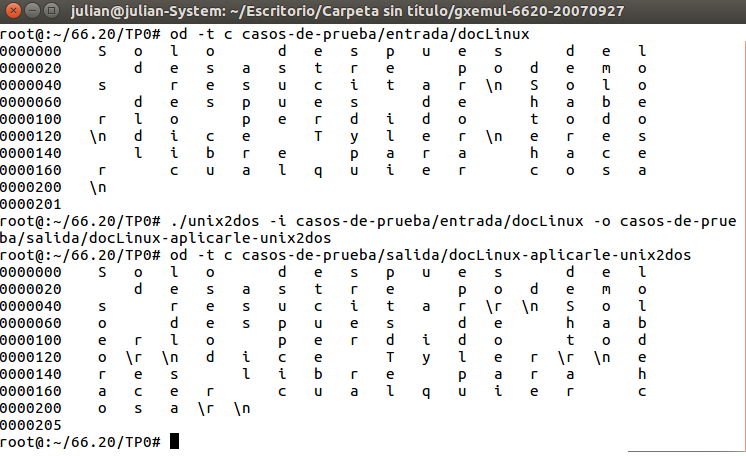
\includegraphics[width=0.8\textwidth]{/casos-prueba/docLinux-aplicarle-unix2dos-salida-archivo.png}
\caption{Prueba de transformar un archivo UNIX a Windows, utilizando archivo de entrada y salida.} \label{fig001}
\end{center}
\end{figure}

\begin{figure}[!htp]
\begin{center}
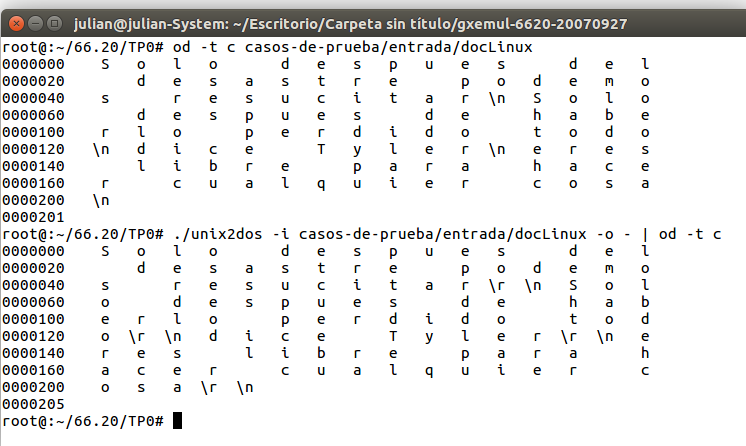
\includegraphics[width=0.8\textwidth]{/casos-prueba/docLinux-aplicarle-unix2dos-salida-estandar.png}
\caption{Prueba de transformar un arhivo UNIX a Windows, utilizando solamente archivo de entrada.} \label{fig001}
\end{center}
\end{figure}

\begin{figure}[!htp]
\begin{center}
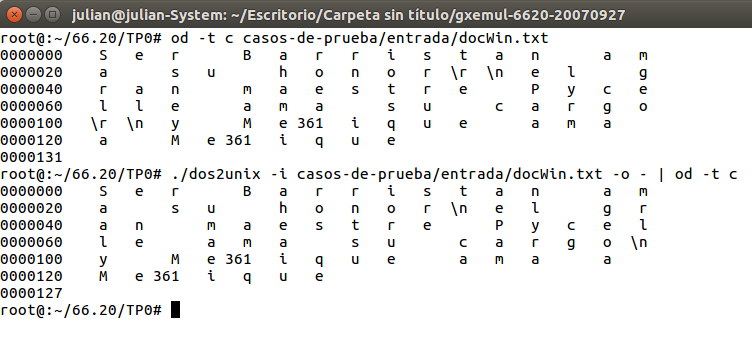
\includegraphics[width=0.8\textwidth]{/casos-prueba/docWin-aplicarle-dos2unix-salida-estandar.png}
\caption{Prueba de transformar un archivo Windows a UNIX, utilizando solo archivo de entrada.} \label{fig001}
\end{center}
\end{figure}

\begin{figure}[!htp]
\begin{center}
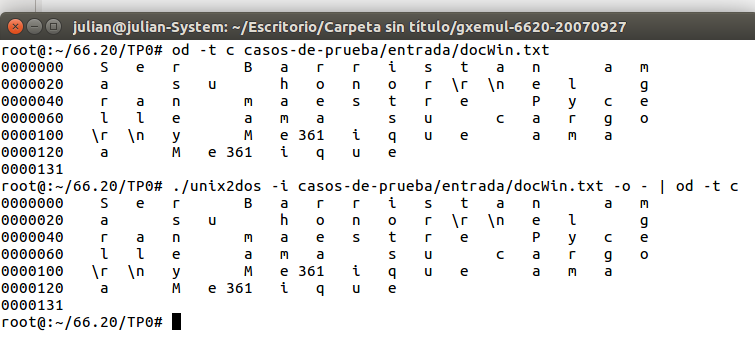
\includegraphics[width=0.8\textwidth]{/casos-prueba/docWin-aplicarle-unix2Dos-salida-estandar.png}
\caption{Prueba de transformar un archivo Windows a un archivo Windows, la salida es la misma.} \label{fig001}
\end{center}
\end{figure}

\begin{figure}[!htp]
\begin{center}
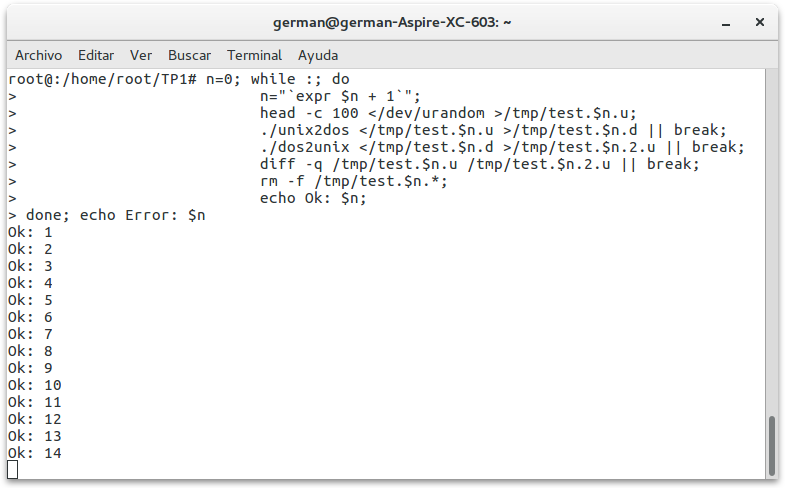
\includegraphics[width=0.8\textwidth]{/casos-prueba/todoOK.png}
\caption{Prueba del programa que genera secuencias de datos aleatorias.} \label{fig001}
\end{center}
\end{figure}

\pagebreak


\section{Conclusiones}

Logramos el objetivo de implementar un conversor de texto capaz de traducir documentos del sistema Unix al de Microsoft y viceversa, que logra pasar todas las pruebas impuestas por la cátedra y las nuestras mediante una implementación que, a nuestros ojos, es limpia y prolija en código Assembly para el sistema MIPS. 

Aplicamos los conceptos dados en clase de forma exitosa, tales como: el uso de funciones, branches y otros más complejos como la correcta segmentación de el stack frame (ABA, LTA y SRA) y el llamado a código propio del sistema operativo mediante la operación de syscall. 

A grandes rasgos, estamos satisfechos con lo obtenido en el presente trabajo, tanto a nivel proyecto como aprendizaje.

\begin{thebibliography}{2}

\bibitem{lib} GetOpt library, 
\texttt{https://www.gnu.org/software/libc/manual/html_node/Example-of-Getopt.html.}

\bibitem{stack} StackOverflow, https://www.stackoverflow.com.

\end{thebibliography}

\end{document}
